\clearpage

\section{FMTDA}\label{sec:FMTDA}\index{FMTDA}

\begin{notebox}
\textbf{Paper: } \fullcite{yao_federated_2022}
\vspace{5pt}

\href{https://openaccess.thecvf.com/content/WACV2022/html/Yao_Federated_Multi-Target_Domain_Adaptation_WACV_2022_paper.html}{reviews not available}
\hspace{1cm}
{No code}
\hspace{1cm}
\href{run:/home/magda/Dropbox/Zot/Yao et al_2022_Federated multi-target domain adaptation.pdf}{Local pdf}
\vspace{3pt}

Presented by Manuel\index{Manuel} in CAIRO readings on 9/2/2022
\hfill Notes taken: 13/2/2022 \index{February 2022}
\end{notebox}

\begin{notebox}[colback=red!5]
\tldr Federated learning\index{federated learning} (FL) setup where server has labelled data and clients have only unlabelled data moreover with shifted data domains. Builds on maximum classifier discrepancy (MCD) [39] training which is a kind of adversarial game with minimax loss where there are two classifiers acting as discriminators and a feature extractor acting as a generator. The generator tries to align the features between the source and target domains and the discriminator step uses two classifiers that try to disagree as much as possible on the target domain while being correct for the source domain. 
In the FL setup they discuss here the problem is all about what is trained where and how it is communicated. Feature extractor needs to be trained on the server together with a global classifier while local classifiers are trained on the clients. The data domains are modelled by a simple GMM which is used to re-weight examples when calculating the classification losses for within and out of distribution data examples.
\end{notebox}

\begin{notebox}[colback=yellow!5]
\textbf{Notes:} 
\begin{itemize}[nosep]
\item Nice paper as not so trivial intro to FL
\item Experiments still surprisingly low accuracy - 30\% on MNIST like data.
\item Possible future work\index{future work}: take on board new clients with new target domains quickly (cannot retrain the whole system every time there is a new client). Use GMMs to find the nearest domain and initialize new client by this classifier. Adapt only client and server and gradually spread?\index{idea}
\end{itemize}
\end{notebox}

\begin{wrapfigure}{r}{0.5\textwidth}
\centering
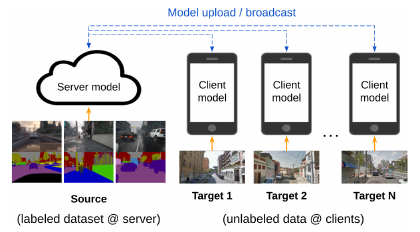
\includegraphics[width=0.5\textwidth]{fmtda_Figure1.png}
% \caption{Federated learning (FL) setup in which the server has labelled data and the clients have unlabelled data. Moreover, the data domains on the server (source domain $D_S$) and the clients (target domains $D_T$) are assumed to be not (perfectly) aligned.}
\end{wrapfigure}
Federated learning (FL) setup in which the server has labelled data and the clients have unlabelled data. Moreover, the data domains on the server (source domain $D_S$) and the clients (target domains $D_T$) are assumed to be not (perfectly) aligned.

Model aggregation on the server in this case won't work because of inter-client discrepancies. Instead they propose dual adaptation approach whereby the models are adapted both at the server and the clients. The models are based on a common feature extractor $G$ and classifier heads $F_i$.

They reuse the maximum classifier discrepancy (MCD) approach introduced in [34 ref in the paper] which has similar minimax game as GAN.
\begin{figure}[ht]
\centering
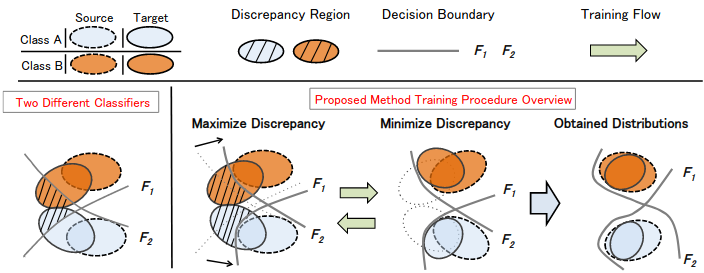
\includegraphics[width=10cm]{fmtda_Figure3.png}
\caption{34 MCD: On one hand train 2 classifiers $F_1$ and $F_2$ that perform well on the source domain but at the same time maximize the classification discrepancy (discriminators) in the target domain. On the other train the feature extractor (generator) to fool the discriminators, that is minimize the discrpancy. This shall push the target features into the source domain.}
\end{figure}
\begin{align*}
\text{Discriminator loss: } \quad & \argmin_{F_1, F_2} \Ls_{ce}(D_S) - \Ls_{adv}(D_T) \\
\text{Generator loss: } \quad & \argmin_{G} \Ls_{adv}(D_T) \enspace , 
\end{align*}
where $\Ls_{ce}(D_S)$ is standard cross-entropy loss over the labelled source domain and is a suitable discrepancy loss such as $L^1$ norm that they use here $\Ls_{adv}(D_T) \E_{\rvx \sim D_T} \Vert F_1(G(\rvx)) - F_2(G(\rvx)) \Vert_1$.
\begin{wrapfigure}{l}{0.5\textwidth}
\centering
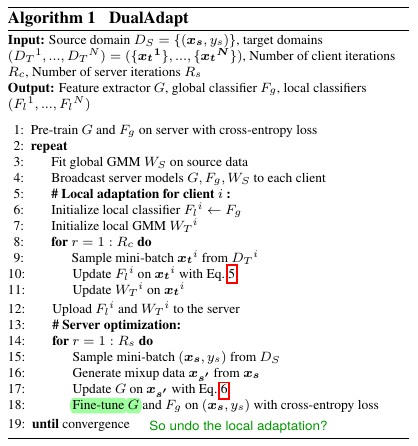
\includegraphics[width=0.5\textwidth]{fmtda_Algo.png}
\end{wrapfigure}

In their setup they update the generator (feature extractor) $G$ on the server and have a global classifier $F_g$ on the server and local classifiers $F_t^i$ on the clients.
They train the local classifiers $f_t^i$ via the discriminator loss by maximizing the $\Ls_{adv}$ discrepancy between the global (fixed here) and local classifiers together with minimizing the cross-entropy using the predictions of the global classifier $F_g$ as the ground truth.
Since the labels from $F_g$ may not be perfect, they use GMM fitted on $D_S$ to re-weight the target examples (if out of source distribution, should have lower weight).

They also fit GMM on the clients. These local GMMs are uploaded together with the local classifiers to the server. The feature extractor $G$ is trained on the server by minimizing the generator loss with $\Ls_{acv}$ evaluated over mix-up instances (simple avg of two randomly sampled instances from $D_S$) weighted by local GMM mixtures. This is done for each target domain so that the server loss is the average across all the target models.

\begin{figure}[ht]
\centering
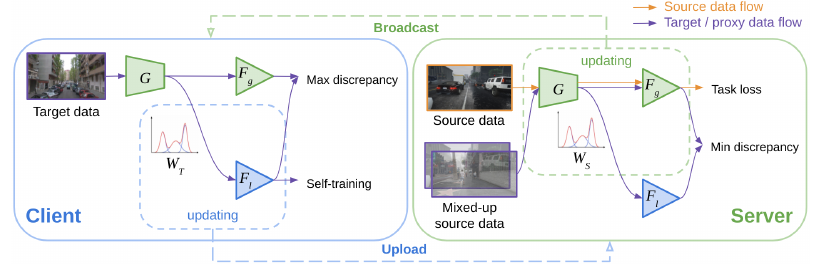
\includegraphics[width=12cm]{fmtda_Figure2.png}
\caption{Dual model adaptation on both clients and server.}
\end{figure}

At inference they classify new instances by averaging the global and local classifier predictions. 

They show experiments on MNIST as the source domain and MNIST-M, SVHN, USPS etc. as targets; DomainNet (clipart, infograph, painting .. )and GTA5 dataset with street-views simulated from computer games. It seems to perform better then baselines though still only about 30\% accuracy on MNIST-like data.

